\section*{Implementation}

FALDO is a small OWL2 ontology which fits in the ALCQ(D) classification difficulty.
It has 14 classes of which 9 deal with the concept of a position on a sequence. 
4 of those classes there to describe accurately what we know of a position that is not precisely determined. 
4 are to deal with the concept of a position on a strand of DNA, e.g. positive, negative and on both strands.
Unlike many representations there is no explicit way to say that it is not ``known'' on which strand a position is,
such an explicit statement can introduce knowledge clashes when merging different datasets.
For example this would lead to positions that are both of the type forward stranded position and a unknown position.
There is also no benefit to explicitly stating that something is unknown as it does not make queries simpler and 
only increases the data size.

The ontology contains only one datatype property: $\mathtt{faldo\colon{}position}$ which is there to give an integer,
a one-based offset from the start of the reference sequence.
This $\mathtt{faldo\colon{}position}$ together with the $\mathtt{faldo\colon{}reference}$ object property links the concept
of a $\mathtt{faldo\colon{}Position}$ to an instance of sequence in the biological sense.
\begin{figure}
\begin{center}
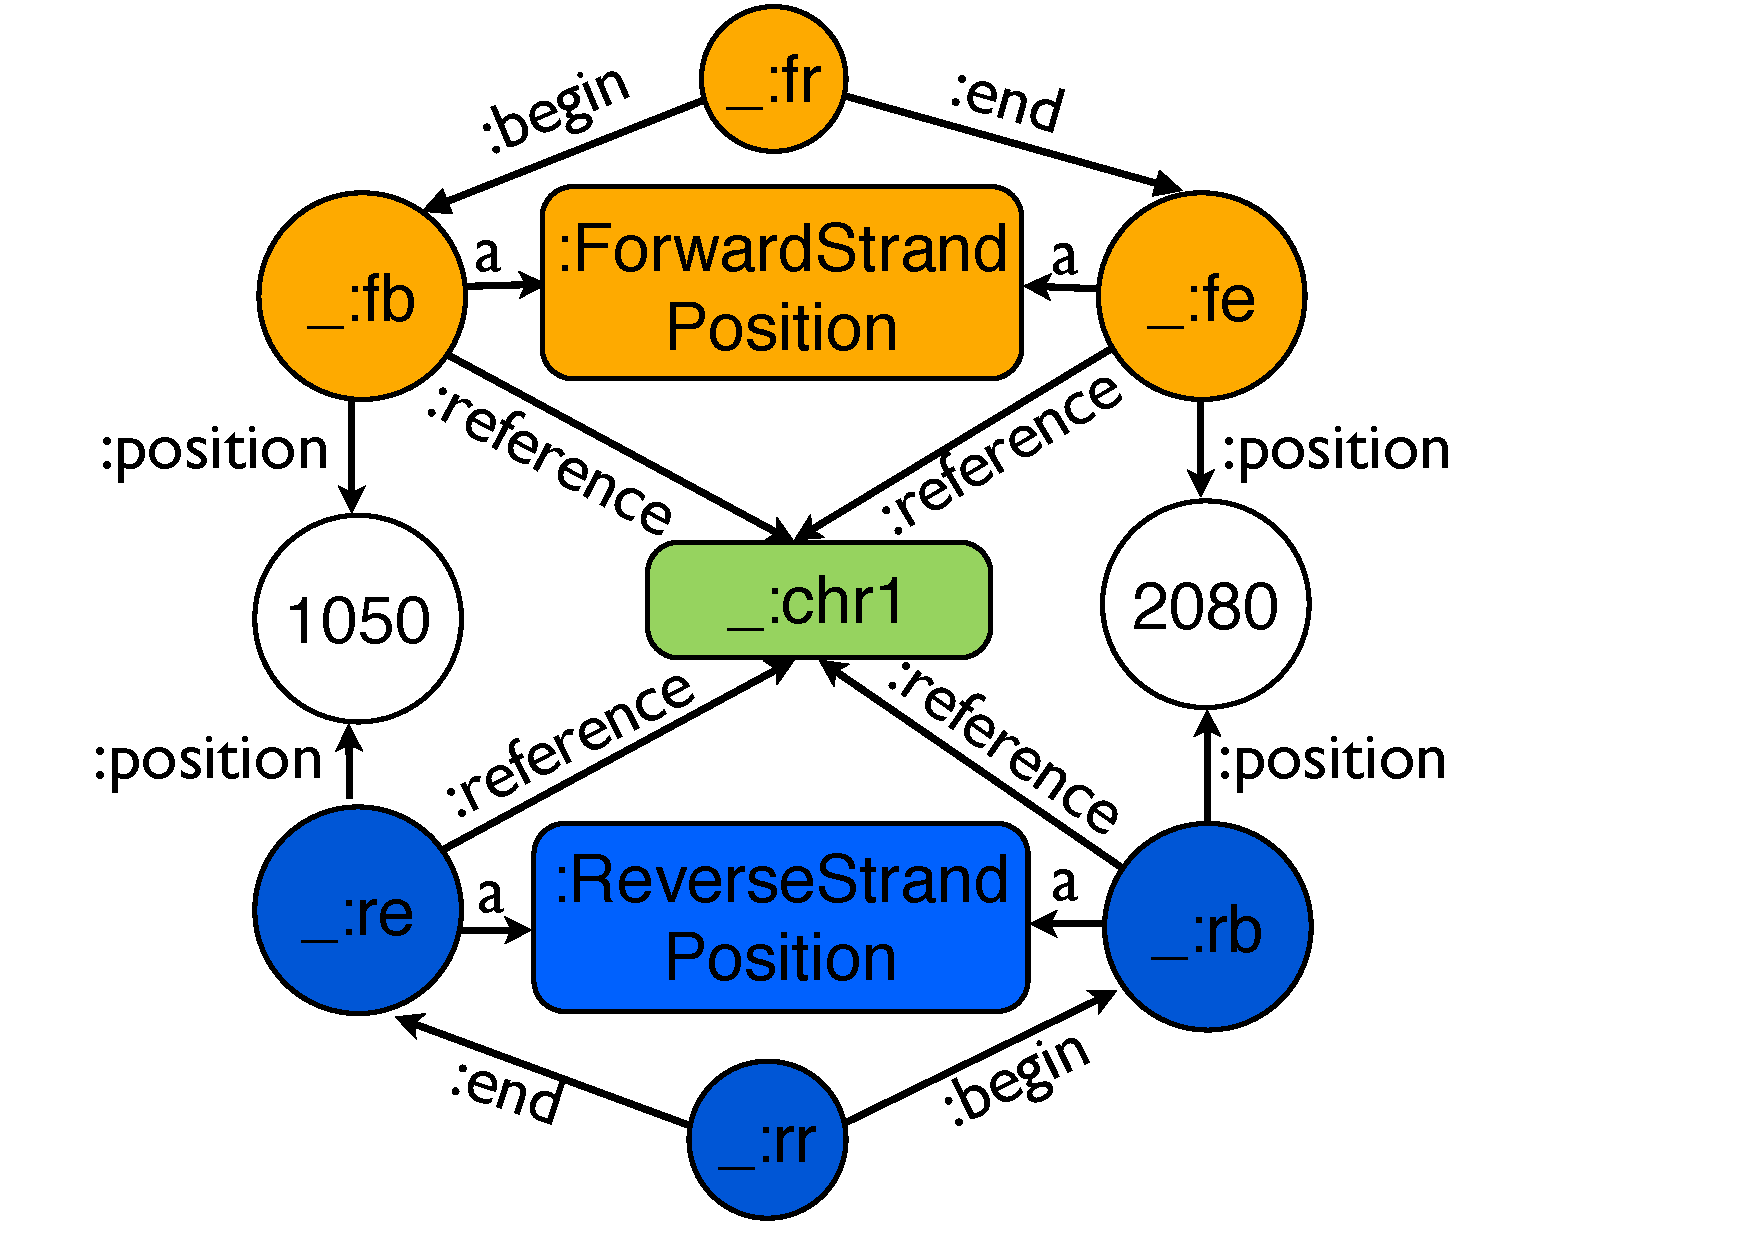
\includegraphics[width=8cm]{figures/figures3.pdf}
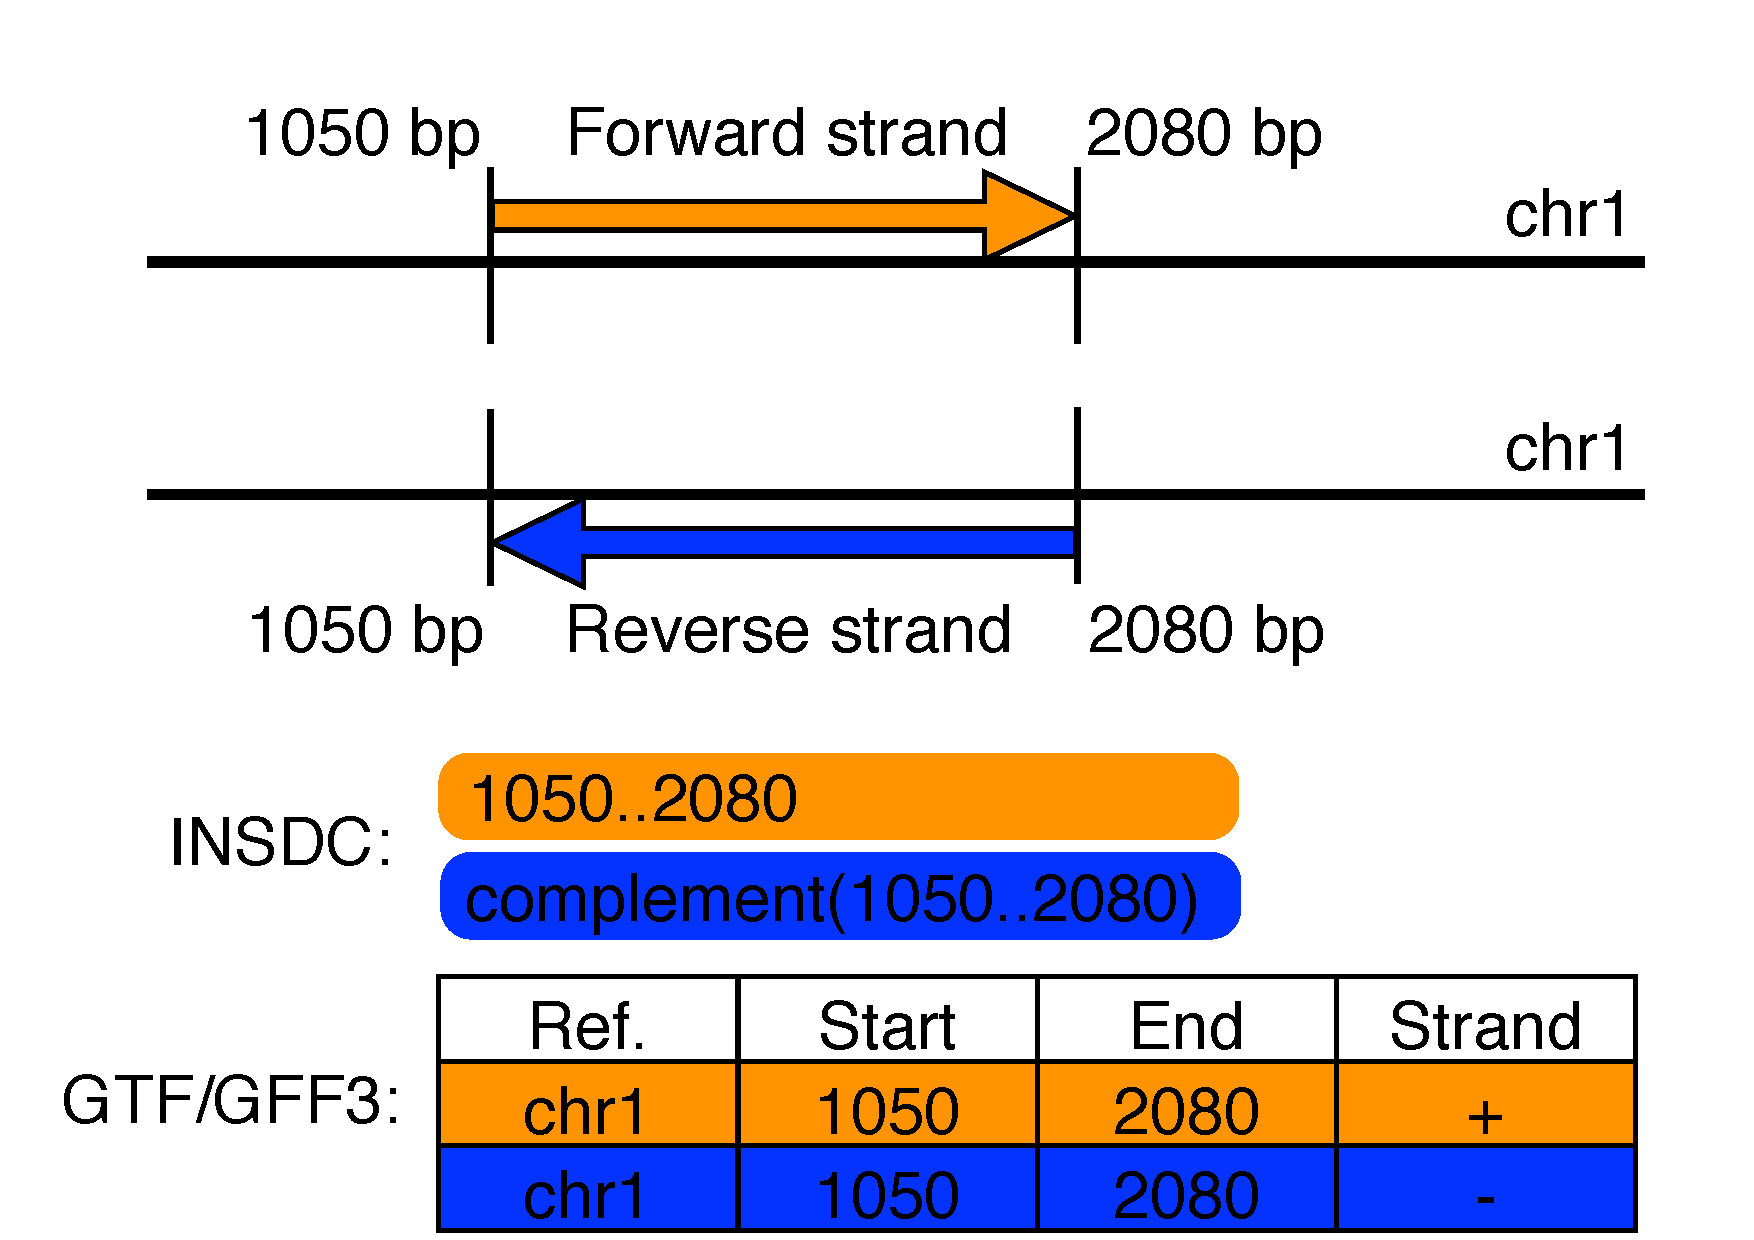
\includegraphics[width=8cm]{figures/figures.pdf}
\end{center}
\caption{Assorted conventions for regions, start, end, and strands.
This figure shows two hypothetical features on a DNA sequence
(labelled \texttt{chr1}), on either the forward strand (orange) or
reverse strand (blue).
Using the INSDC location string notation, these regions are
``\texttt{1050..2080}'' and ``\texttt{complement(1050..2080)}''
respectively if implicitly given in terms of the reference chr1.
Using the GTF/GFF3 family of formats, regardless of the
strand these two locations are described with $start = 1050$
and $end = 2080$, and in general, $start \leq end$.
Biologically speaking, in terms of transcription, the start of a genomic
feature is strand dependent.
For the forward strand feature (orange), the start is 1050
while the reverse strand feature (blue) starts from 2080.}
\label{fig:strands}
\end{figure}

\subsection*{OWL2 reasoning based compression}
For large databases such as INDSC or UniProt the need to repeat the reference sequence for positions again and again may incur a significant cost in storage.
However, this triple does not need to be materialised in the database as it is inferable using OWL2 property chain reasoning.
With the axiom shown in fig:\ref{owl:chainProperty} the $\mathtt{faldo\colon{}reference}$ triples can be inferred for any $\mathtt{faldo\colon{}position}$ described by a INSDC record.
\begin{figure}
\begin{shaded}
\small
\begin{verbatim}
INDSC:reference
      a       owl:ObjectProperty ;
      rdfs:subPropertyOf faldo:reference ;
      owl:propertyChainAxiom
              (faldo:endOf faldo:locationOf INDSC:featureOf INDSC:sequence) , 
              (faldo:locationOf INDSC:featureOf INDSC:sequence) , 
              (faldo:beginOf faldo:locationOf INDSC:featureOf INDSC:sequence) .

\end{verbatim}
\end{shaded}
\caption{OWL2 property chain axiom to infer that all positions described in a INSDC record are positioned relative to the main sequence of the record (in RDF turtle syntax).}
\label{owl:chainProperty}
\end{figure}
A OWL capable query rewriter means that users do not see the difference between encoding the $\mathtt{faldo\colon{}reference}$ explicitly or having them inferred at query time.
For RDF databases that do not have such capabilities can easily add the necessary triples using a single SPARQL insert query as shown in fig:\ref{sparql:chainProperty}. This flexibility in solving this problem allows users of the data to use the best approach for their infrastructure instead of being limited by the decisions of the data provider.
\begin{figure}
\begin{shaded}
\small
\begin{verbatim}
INSERT {
    ?position faldo:reference ?sequence .
}
WHERE {
    ?record a insdc:Entry ;
            insdc:feature ?feature ;
            insdc:sequence ?sequence .
    ?feature faldo:location ?location .
      { ?location faldo:begin|faldo:end ?position . }
    UNION
      { ?location a faldo:Position . }
}
\end{verbatim}
\end{shaded}
\caption{SPARQL query to add all $\mathtt{faldo\colon{}reference}$ properties to $\mathtt{faldo\colon{}positions}$ described from a $\mathtt{insdc\colon{}record}$.}
\label{sparql:chainProperty}
\end{figure}

\subsection*{Validating a FALDO model}

Some databases only allow a subset of all FALDO. For example
INSDC requires that the start and end of a region are on the same sequence 
and UniProt requires that a feature is described in relation to the canonical isoform.
Semantic technology gives a number of different options\cite{RDFValidationReport} to add 
such optional constraints to a datamodel. 
The benefit of such optionality is that constraints needed for quality control at 
the data provider do not restrict the users of the data in any way. 

For example the UniProtKB constraint that positions are annotated on the canonical isoform 
(for comparability with legacy data formats), if enforced, may make it difficult for a proteomics
database describing a glycosylation site that is specific to a single isoform described in UniProtKB.

\subsection*{Users}
FALDO is implemented and used in a number of tools and databases.

\begin{description}
\item[JBrowse sparql] FALDO is used in sparql queries determine where to draw information related to a reference sequence in tracks filled with data from semantic databases. 
\item[INSDC-DDBJ] DDBJ is currently working on a RDF format for the INSDC data that is stored in DDBJ/GenBank/EMBL-Bank.
\item[BioInterchange] uses FALDO to make position information in current bioinformatics data stored in files such as GTF or GFF3 available to the semantic web (\url{http://www.biointerchange.org/}).
\item[TogoGenomes] a bacterial genome database collection provided by the DBCLS also uses FALDO in its RDF representation (\url{http://togogenome.org/}).
\item[Intermine] The popular model organism database software collection uses FALDO in its SPARQL mode.
\item[phenomebrowser] Positions of phenotypes and disease related natural variations are positioned onto the Mouse genome using FALDO.
\item[BOING] The ``bio-ontology integrated querying of sequence annotations'' also uses FALDO to describe all feature locations \cite{BOING}.
\item[SPARQL-bed] This simple tool that turns any BED file into a web accessible SPARQL endpoint also uses FALDO to describe BED feature positions (\url{https://github.com/JervenBolleman/sparql-bed}).
\item[BioBerl] BioPerl\cite{BioPerl2002} now includes a FALDO exporter (Bio::FeatureIO::faldo), which allows any bioperl feature format to be translated to FALDO.
\item[UniProt] UniProt annotates many protein features and sites. Starting with UniProt RDF release 2013$\_$11 the positions of a protein feature is described using FALDO.
\end{description}


